% Self-contained LaTeX source; no external figure files are required.
% Compile with pdfLaTeX (e.g. Overleaf's default compiler).
% Run commands in the report from the Python project root.
% Measurements are from results/scalability/benchmark.json, not new runs.
\documentclass[11pt,a4paper]{article}
\usepackage[margin=23mm]{geometry}
\usepackage[T1]{fontenc}
\usepackage{lmodern}
\usepackage{microtype}
\usepackage{amsmath}
\usepackage{booktabs,tabularx}
\usepackage{xcolor,listings}
\usepackage{pgfplots}
\pgfplotsset{compat=1.18}
\usepackage[hidelinks]{hyperref}
\usepackage{url}
\lstset{basicstyle=\ttfamily\footnotesize,breaklines=true,
  columns=fullflexible,keepspaces=true,showstringspaces=false,
  frame=single,rulecolor=\color{black!20},aboveskip=6pt,belowskip=6pt}
\setlength{\parindent}{0pt}
\setlength{\parskip}{5pt}
\setlength{\emergencystretch}{2em}
\title{Finding Textually Similar Documents\\
  \large Shingling, MinHash, and Locality-Sensitive Hashing}
\author{} % Add your name and student ID here.
\date{16 November 2026}

\begin{document}
\maketitle
\vspace{-1.5em}

\section{Solution}
The Python project implements all five assignment stages, including LSH.
\path{shingling.py} normalizes text and converts unique overlapping
10-character shingles into stable 64-bit BLAKE2b hashes. It also computes
exact Jaccard similarity, $J(A,B)=|A\cap B|/|A\cup B|$; documents are
similar when $J\geq0.8$.

\path{minhashing.py} constructs 120-component signatures by taking the
minimum value of each hash function (seed 42). Signature similarity is
the fraction of matching components. \path{lsh.py} uses 12 bands of
10 components: a match in any corresponding band creates a candidate pair.
Candidates are deduplicated and their signatures compared. LSH is
approximate and may miss similar pairs. \path{pipeline.py} integrates the
stages, while \path{io_utils.py} and \path{cli.py} handle input and execution.

\section{Build and run instructions}
Python 3.9 or later is required; the algorithm uses only the standard
library and needs no compilation. From the project root:
\begin{lstlisting}
python3 -m pip install -e .
similar-items analyze --input data/election_2026/corpora/scale_10 \
  --output results/sample_analysis.json
\end{lstlisting}
The CLI prints similar pairs and evaluation metrics, and optionally saves
JSON. In PyCharm, run \path{main.py}; its default corpus is
\path{data/election_2026/corpora/real_20}.

\begin{center}
\small
\begin{tabularx}{\linewidth}{@{}llX@{}}
\toprule
\texttt{analyze} parameter & Default & Meaning \\
\midrule
\texttt{--input} & Required & Directory containing UTF-8 \texttt{.txt} files. \\
\texttt{--k} & 10 & Character shingle length; positive integer. \\
\texttt{--num-hashes} & 120 & Signature length; positive integer. \\
\texttt{--threshold} & 0.8 & Similarity threshold in $[0,1]$. \\
\texttt{--seed} & 42 & Seed used to generate the MinHash functions. \\
\texttt{--bands} & Automatic & Positive divisor of signature length. \\
\texttt{--output} & None & JSON destination; omitted means no output file. \\
\bottomrule
\end{tabularx}
\end{center}

The final dataset is supplied separately as
\texttt{election\_2026\_1000.zip} through a cloud drive; texts and the
distribution archive are excluded from Git. Download it from the
\href{https://drive.google.com/drive/folders/12gJchd3Gv5oO9GsbdZrfX5CRR0VNfaGZ}{Google Drive dataset folder}
and import it
before analysis (replace the example path):
\begin{lstlisting}
python3 scripts/dataset_archive.py import \
  --archive /path/to/election_2026_1000.zip
\end{lstlisting}
\texttt{--archive} is required. The standard-library importer verifies
SHA-256 hashes and restores the original 10-, 100-, and 1000-document
corpora and the 20-article example under
\path{data/election_2026/corpora/}. The ZIP stores each final text once;
subsets follow the repository manifests. No web collection or variant
regeneration is required. Download details are maintained in
\path{data/election_2026/DOWNLOAD.md}.

Run the unit tests and reproduce the scalability experiment with:
\begin{lstlisting}
PYTHONPATH=src python3 -m unittest discover -s tests -v
python3 scripts/benchmark_scalability.py --repeats 3
\end{lstlisting}
\texttt{--repeats} defaults to 3. The benchmark fixes corpus sizes at
10, 100, and 1000 and uses the algorithm defaults above. Use this script
for timing: the interactive CLI additionally evaluates all document pairs.

\section{Dataset and measurement protocol}
The November 2026 US midterm-election corpus contains 200 real texts
(44 articles and 156 live-blog updates) from CBS News, The Guardian,
AP, and Roll Call, predominantly CBS. Each original has four variants
created by sentence deletion or adjacent-sentence swaps. Thus, the largest
input contains \emph{200 real texts and 800 synthetic variants}, not
1,000 independent articles. Smaller corpora are nested subsets containing
complete five-document families.

\begin{center}
\small
\begin{tabular}{@{}rrrrr@{}}
\toprule
Documents & Originals & Variants & Total words & Total shingles$^{*}$ \\
\midrule
10   & 2   & 8   & 2,470   & 13,101 \\
100  & 20  & 80  & 23,900  & 130,707 \\
1000 & 200 & 800 & 243,225 & 1,325,505 \\
\bottomrule
\end{tabular}

\footnotesize $^{*}$Sum of the unique-shingle counts of individual documents.
\end{center}
Measurements used Python 3.9.6 on Darwin 24.6.0 (x86\_64), in one process
without explicit parallelism. After an excluded 10-document warm-up,
each size was run three times, rebuilding all representations.
\texttt{time.perf\_counter()} measured wall-clock time; results are medians.

\textbf{Algorithm time includes setup, shingling, MinHash, LSH, and
candidate signature comparison only.} File I/O, every exact Jaccard
calculation, quality evaluation, and plotting are excluded.
Exhaustive Jaccard evaluation afterward supplies ground truth, including
cross-family pairs.

\section{Results and discussion}
Table~\ref{tab:times} shows algorithm-only times. Independent stage
medians need not sum to the median total, which is computed per trial.

\begin{table}[htbp]
\centering\small
\caption{Algorithm execution time in seconds: median of three trials.}
\label{tab:times}
\begin{tabular}{@{}rrrrrrr@{}}
\toprule
$N$ & Setup & Shingling & MinHash & LSH & Sig. compare & Total \\
\midrule
10 & 0.000380 & 0.028391 & 0.746020 & 0.000206 & 0.000174 & 0.775058 \\
100 & 0.000398 & 0.276657 & 7.354960 & 0.008219 & 0.001416 & 7.646833 \\
1000 & 0.000390 & 2.961405 & 74.846946 & 0.090827 & 0.018505 & 77.926033 \\
\bottomrule
\end{tabular}
\end{table}

\begin{figure}[htbp]
\centering
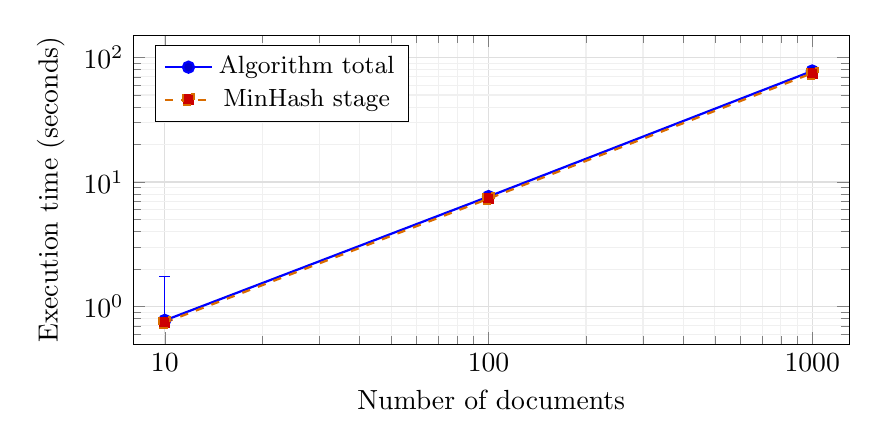
\begin{tikzpicture}
\begin{loglogaxis}[
  width=0.88\linewidth,height=5.5cm,
  xlabel={Number of documents},ylabel={Execution time (seconds)},
  xtick={10,100,1000},xticklabels={10,100,1000},
  xmin=8,xmax=1300,ymin=0.5,ymax=150,
  grid=both,minor grid style={gray!12},major grid style={gray!25},
  legend pos=north west,legend style={font=\small},
]
\addplot+[blue,mark=*,thick,error bars/.cd,
  y dir=both,y explicit]
  table[x=n,y=t,y error minus=lo,y error plus=hi] {
  n t lo hi
  10 0.775057619 0.015296013 0.957645116
  100 7.646833396 0.031912945 0.191549729
  1000 77.926033322 1.241081471 0.580646031
};
\addlegendentry{Algorithm total}
\addplot+[orange!85!black,mark=square*,dashed,thick]
  coordinates {(10,0.746019953) (100,7.354959503) (1000,74.846946252)};
\addlegendentry{MinHash stage}
\end{loglogaxis}
\end{tikzpicture}
\caption{Algorithm-only time (logarithmic axes). Error bars show observed
minima and maxima over three runs, not confidence intervals.}
\label{fig:scaling}
\end{figure}

A tenfold input increase raised median time by factors of 9.87 and 10.19,
showing approximately linear growth over the measured sizes. MinHash
accounted for about 96\% of the largest run's median algorithm time.

\begin{table}[htbp]
\centering\small
\caption{LSH candidates evaluated against exact Jaccard at $s=0.8$.}
\label{tab:quality}
\begin{tabular}{@{}rrrrrrr@{}}
\toprule
$N$ & True pairs & Candidates & Retrieved true & Precision & Recall & Pair reduction \\
\midrule
10 & 9 & 12 & 9 & 75.00\% & 100.00\% & 73.33\% \\
100 & 85 & 105 & 74 & 70.48\% & 87.06\% & 97.88\% \\
1000 & 921 & 1,175 & 876 & 74.55\% & 95.11\% & 99.76\% \\
\bottomrule
\end{tabular}
\end{table}

Precision is the fraction of candidates that are truly similar; recall
is the fraction of all true pairs retrieved. Pair reduction compares
candidate count with all possible pairs, not elapsed time. At 1000
documents, LSH reduced 499,500 possible pairs to 1,175 candidates and
retrieved 876 of 921 true pairs. Exact verification removes false positives
but cannot recover the 45 missed pairs; its time is excluded above.

These results apply to this synthetic-augmented corpus and fixed seed;
three repetitions measure timing variation, not variation across hash
families. Raw measurements and detailed pair results are available in
\path{results/scalability/}; source provenance and corpus manifests are
under \path{data/election_2026/}.

\end{document}
